\section{Experiment}

\subsection{Comparison between categorical smoothing and Laplace smoothing}

\begin{table}[t]
\caption{Precision Comparison between categorical smoothing and Laplace smoothing}
\label{tab-smoothing-comparison}
\vskip 0.15in
\begin{center}
\begin{small}
\begin{sc}
\begin{tabular}{l|cc|c}
\hline
\abovespace\belowspace
Data set & Laplace & categorical & improvement \\
\hline
\abovespace
Top 1k set & 0.5906 & 0.8764 & 0.2858 \\
\belowspace
Lower 1k set & 0.6455 & 0.8128 & 0.1673 \\
\hline
\end{tabular}
\end{sc}
\end{small}
\end{center}
\vskip -0.1in
\end{table}

\begin{figure}[ht]
\vskip 0.2in
\begin{center}
\centerline{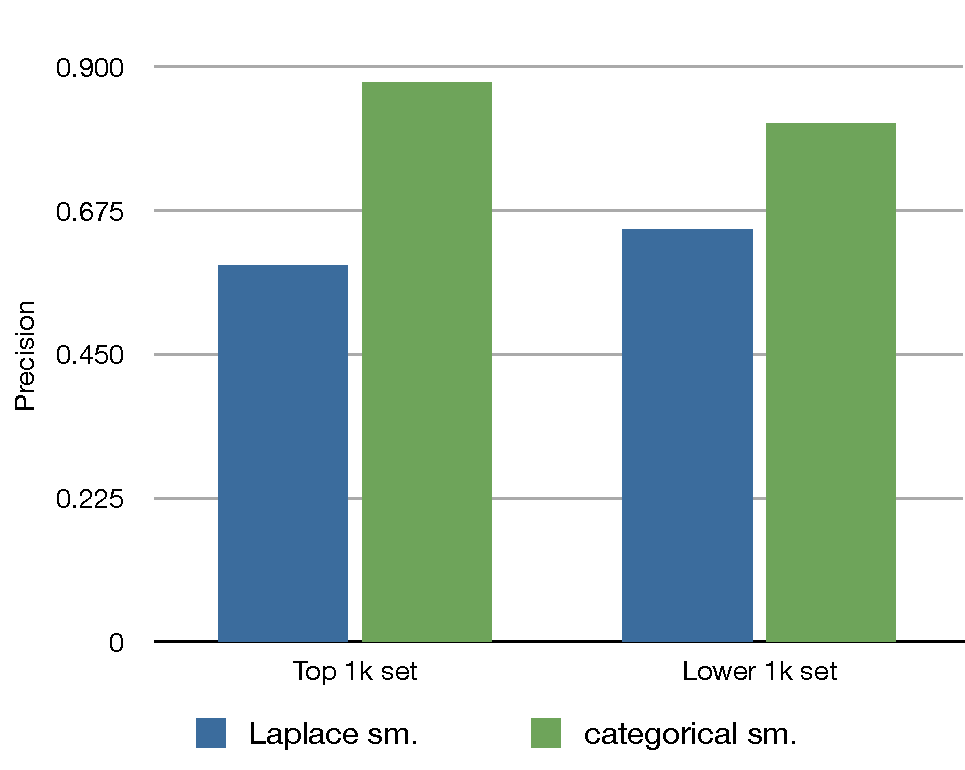
\includegraphics[width=\columnwidth]{pvssmoothing}}
\caption{Precision Comparison between categorical smoothing and Laplace smoothing}
\label{fig-p-vs-smoothing}
\end{center}
\vskip -0.2in
\end{figure}

We use two different verb sets to compare the effect of categorical smoothing and Laplace smoothing. One set is the top 1000 most frequent unstemmed verbs in the SVO tuple corpus, the other lower 1000 set is the 10001st to 11000th most frequent unstemmed verbs in the SVO tuple corpus. The top 1000 set contains 538 unique stemmed verbs while the lower 1000 set contains 935 unique stemmed verbs. However, the number of examples in training and testing set are quite different. The top 1000 set has about 206k testing examples while the lower 1000 set has 18.9k testing examples. The numbers of training set have the same proportion.

From the comparison result in \ref{tab-smoothing-comparison} and \ref{fig-p-vs-smoothing}, we see that categorical smoothing provides a significant improvement on the precision on both datasets. It improves the precision on top 1000 set for 0.2858 and lower 1000 set for 0.1673 respectively. We also observe that the improvement of categorical smoothing is more significant on the top 1000 set than on the lower 1000 set.

One thing we must mention is the high disk space cost during the Hadoop testing procedure. On the test set with only 261894 test cases and top 1000 label set, the disk cost is over 30GB, and the processing time is over 1 hour on a laptop. In the testing procedure, we need to emit s-v and v-o pairs for all possible verbs for each test case. Given there are only two features in each document, the disk cost is estimated as $O(verb\_set\_size * number\_of\_test\_cases)$. 

\subsection{Comparison between Unigram Prior and Uniform Prior}

\begin{table}[t]
\caption{Precision Comparison between Unigram Prior and Uniform Prior}
\label{tab-prior-comparison}
\vskip 0.15in
\begin{center}
\begin{small}
\begin{sc}
\begin{tabular}{l|cc}
\hline
\abovespace \belowspace
Data set & Top 100 set & Lower 100 set \\
\hline
\abovespace
unigram prior & 0.8603 & 0.6376 \\
\belowspace
uniform prior & 0.9314 & 0.7784 \\
\hline
\abovespace
\belowspace
Difference & 0.0711 & 0.1408 \\
\hline
\end{tabular}
\end{sc}
\end{small}
\end{center}
\vskip -0.1in
\end{table}

Based on the Naive Bayes formula, $P(v)$ is the prior probability to predict the verb $v$. In unigram prior, the term is set as $doc_count(v) / total_doc_count$. But in uniform prior, it's set to $1/number_of_unique_verbs$, then canceled in the formula, in which case the formula becomes:

\begin{equation}
	\hat{v} = \arg\max_v p(s|v)p(o|v)
\end{equation}

Table \ref{tab-prior-comparison} shows the results of comparison experiments for both priors on two different label set settings. One label set is the top 100 most frequent unstemmed verbs which contains 68 unique stemmed verbs. The other label set is the 1001st to 1100th most frequent unstemmed verbs which contains 96 unique stemmed verbs. From the results, we see that uniform prior performs better than unigram prior on both label set settings. 

The experimental result from comparison between unigram prior and uniform prior is confusing. Unigram model is expected to be a better model than the pure random guessing uniform model. when used as a prior, given other factors are fixed, unigram model should result in a better result. However it's not the truth from our repeating experiments on different label sets. The two experiments on different label sets got $7\%$ and $14\%$ percent improvement on precision when we change the unigram prior to uniform prior. One observation is that when unigram prior is added, the prediction always prefer those popular verbs like "is" and "have". Even if we remove these verbs as "stop words", the result is still not as good. Though we still can't interpret the reason why uniform prior is better, in our bast model, uniform prior is used. \cite{peng2004augmenting}

\subsection{Smoothing Parameter}

\begin{figure}[ht]
\vskip 0.2in
\begin{center}
\centerline{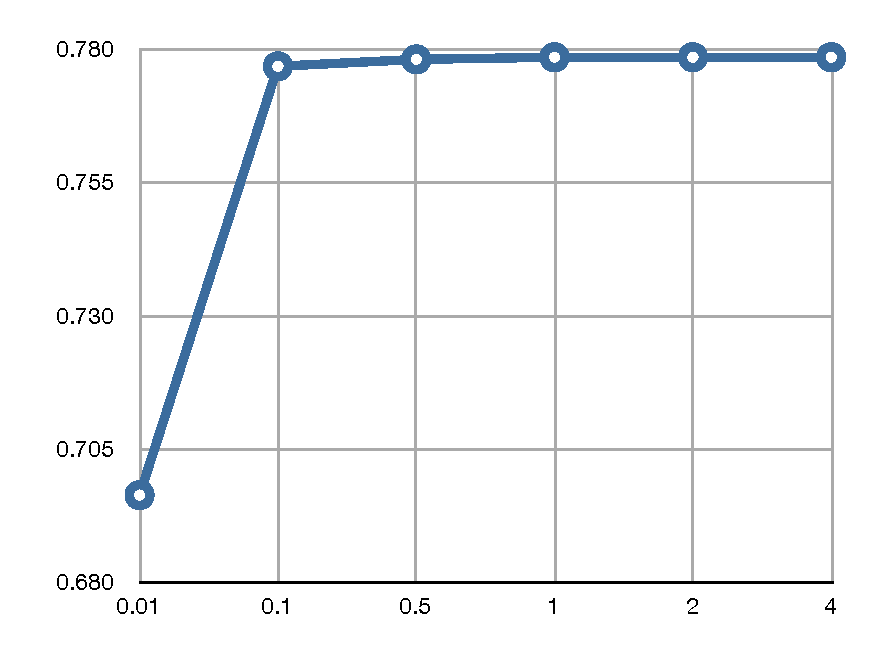
\includegraphics[width=\columnwidth]{pvsalpha}}
\caption{Precision vs. Smoothing parameter in Categorical Smoothing}
\label{fig-p-vs-alpha}
\end{center}
\vskip -0.2in
\end{figure}

We tuned the smoothing parameter $\alpha$ manually with several different values. When $\alpha$ is set to one, it is similar to Laplace smoothing but works on categorical counts instead of global vocabulary size. When $\alpha$ gets larger, the effect of category information is enlarged. From Figure \ref{fig-p-vs-alpha}, we find that when $\alpha$ is extreme small, the precision is decreased. When alpha increases, the precision generally increase, however, when alpha is larger than one, the precision is fixed on 0.7784 and never increases no matter how large it is set to.

We tried $\alpha=0$, and the experiment didn't success because of the zero probability product doesn't make sense. We tried to remove conditional probability of words and keep only the category based probability, but we got only a 0.0188 precision which is like random guess. We also had controlled experiments with Laplace smoothing with $\alpha=1$ and got the precision 0.6074, which is much lower than any alpha settings in categorical smoothing. 



